%!TEX root = ../username.tex
\chapter{Background} \label{bg}

% TODO write an introduction to this section

\section{Musical Terminology and Notation} \label{bg:musicTerminology}

This paper contains the some musical terminology which not all readers may be familiar with.
This section contains definitions of musical terms that are important to fully understand the rest of the paper.

\textbf{Beat}: The beat is the fundamental unit of rhythm.
What a beat looks like is context dependent.
For example, in one piece the beat may be the quarter note, in a second piece it may be a dotted quarter note, in a third piece it might be the half note.
A tempo (speed) is generally provided to determine how long each beat should last.
This may take the form of a specific number of beats per minute or a more general term, such as \textit{Allegro} for fast, or \textit{Largo} for slow.
The beat can be multiplied or divided into smaller parts to create different rhythms.

\textbf{Chord}: A chord consists of several notes played as a single unit.
Most commonly, three or more notes are played simultaneously, though two notes may also constitute a chord.
Common chords are based on the major and minor scales, with variations depending on the order of the notes from lowest to highest.

\textbf{Chord tone}: A chord tone is a note contained in a chord.
For example, C, E, and G are chord tones of a C Major chord.

\textbf{Harmony}: Harmony consists of all the notes played at the same time as the melody that are not part of the melody.
In Western music, these harmonies generally follow a progression of chords based on the key that enhance the melody.

\textbf{Key}: The key of a piece of music determines the chords that appear, as well as the scale the music generally follows.
The name of a key takes the form of <Pitch> <Modifier>, where the pitch is one of fifteen pitches, and the modifier specifies the mode of the key, most ofter Major or Minor.
The pitch indicates the starting pitch of the scale.
Key is notated by the key signature on the music staff, a set of sharps or flats on specific lines and spaces.

\textbf{Measure}: In music, a measure is a collection of notes grouped together in order to give a piece some structure.
Measures within a piece generally contain the same number of beats.

\textbf{Melody}: The melody is the most prominent part, often played in the highest voice.
It is the recognizable tune that generally defines a piece of music.

\textbf{MIDI}: (Musical Instrument Digital Interface) This is a standard that defines a digital interface, communication protocol, and electrical connectors that allows computers, electronic instruments, and other audio devices to communicate.

\textbf{Non-chord tone}: A non-chord tone is a note that appears while a chord is played but is not part of the chord.
Non-chord tones may be used to insert dissonance and drive a piece of music toward resolution.
For example, F is a non-chord tone when played over a C Major chord.

\textbf{Note length/rhythm}: Durations of notes used to indicate how much of each beat a note should occupy and are divided as follows:
The quarter note (\quarternote) is often the most basic division of the beat, at one quarter note per beat.
The eight note (\eighthnote) is half the duration of the quarter note, while the half note (\halfnote) is double the duration of the quarter note, and the whole note (\fullnote) is four times the duration.
The names for these note lengths come from how many of that type of note can fit in a common time measure (which lasts for one whole note, or more often four quarter notes).
These durations continue in ether direction, so there exist sixteenth and thirty-second notes, as well as double whole notes.
Dots can also be applied to notes to add half the duration of the base note.
For example, a dotted quarter note (\quarternote.) takes the same amount of time as three consecutive eighth notes (\eighthnote \eighthnote \eighthnote).

\textbf{Pitch classes}: When two notes have the same letter, but are not necessarily in the same octave, they have the same pitch class.
When discussing the harmonic structure of music, notes of the same pitch class are equivalent, so the octaves in which notes appear do not change the harmonic structure.

\textbf{Scale}: A scale is a way of choosing which notes to include in a piece and is closely related to the concept of a key.
Scales begin on one pitch class, and ascend one octave before repeating.
Different modes have different feelings.
For example, the major mode (Ionian) sounds more bright and happy, while the minor modes (Aeolian, Dorian, and Phrygian) sound more dark and sad.

\textbf{Tonic}: The tonic pitch is the base note of a scale.
For example, in the C Major scale, C is the tonic.

\section[Markov Chains]{Markov Chains} \label{bg:markov}

Intuitively, we may think of a Markov chain as a machine that accepts some former state or states of a system and produces the next state in the system.
The decision of what the next state should be is based on probabilities of transitioning to different states from the current state of the system.

\subsection{Definition} \label{bg:markov:definitions}

More formally, a \textit{Markov chain} is a type of discrete-time stochastic process, which means a Markov chain is a sequence of random variables $\boldsymbol{X} = \{X_{n} | n \in I\}$ for some index set $I$.
Additionally, Markov chains have the special property that they depend only on the immediate past state(s).
That is, for a first-order Markov chain at time $t$, $$P(X_{t} = j \mid X_{0} = i_{0}, \ldots, X_{t - 1} = i_{i - 1}) = P(X_{t} = j \mid X_{t - 1} = i_{t - 1})$$ for a particular possible outcome $j$ of $X_{t}$ \cite{nierhaus_algorithmic_2009}.

This idea can also extend to higher-order Markov chains.
A higher-order Markov process considers more than the single most recent state to determine the next state.
An $n$th order Markov chain uses the previous $n$ states as the input to find the next state.

\subsection{Representations} \label{bg:markov:representations}

In the case when $n = 1$, we can think of a Markov chain as a directed graph, where each state is a node, each edge is a transition between states, and the probabilities of transitioning between states are represented by the edge weights.
See Figure \ref{fig:markovGraph} for a visual representation of this idea.

\begin{figure}[h]
	\centering
	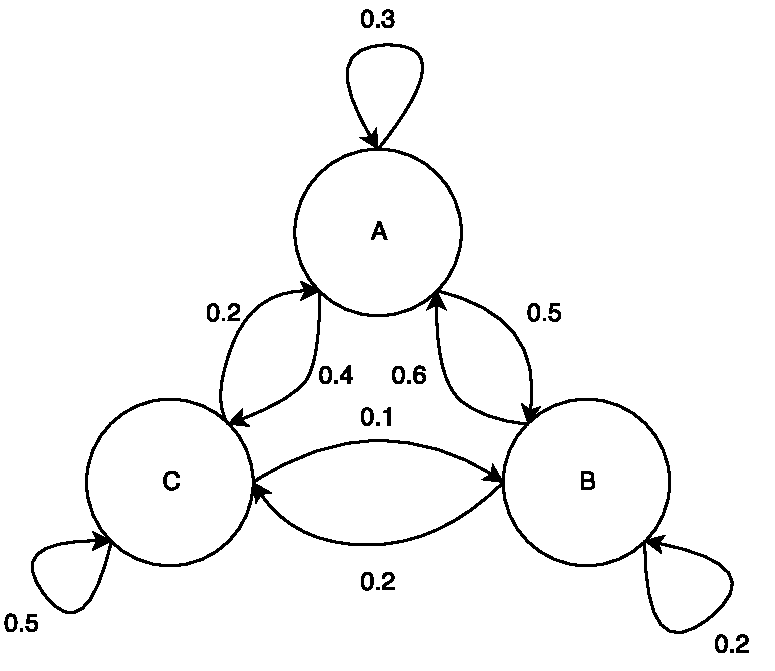
\includegraphics[width=\linewidth]{figures/markovGraph.pdf}
	\caption[A Markov chain represented as a graph.]{A Markov chain represented as a graph. Arrows between nodes represent transitions between nodes.}
	\label{fig:markovGraph}
\end{figure}

When implementing a Markov chain in code, however, it is perhaps easier to represent it as an $(n + 1)$-dimensional array, where $n$ is the order of the Markov chain.
We call this $(n + 1)$-dimensional array the \textit{transition matrix}.
It contains the probabilities of transitioning from one state to another.
See Figure \ref{fig:markovMatrix} for an example of the same Markov chain as in Figure \ref{fig:markovGraph} in matrix form.
Note that the matrix representation is essentially an \textit{adjacency matrix} of the graph, where edge weights are the probabilities of transitioning between nodes.

\begin{figure}[h]
	\centering
	\begin{tabular}{c | c c c}
		& $A_{1}$ & $B_{1}$ & $C_{1}$\\
		\hline
		$A_{0}$ & $0.3$ & $0.5$ & $0.2$\\
		$B_{0}$ & $0.6$ & $0.2$ & $0.2$\\
		$C_{0}$ & $0.4$ & $0.1$ & $0.5$
	\end{tabular}
	\caption[A Markov chain represented as a transition matrix.]{A Markov chain represented as a transition matrix. Rows represent transitions from the labeling node to the labeling node of each column.}
	\label{fig:markovMatrix}
\end{figure}

\subsection{Limitations} \label{bg:markov:limitations}

A major limitation of Markov chains is their inability to generate truly novel output.
In order for some state to appear, a transition to that state from the previous state must appear in the \textit{source material}, the set of data from which the transition probabilities come.
That is, no truly novel transitions may appear; all transitions that appear in the output of the Markov chain must have appeared somewhere before.
Additionally, lower-order chains may produce nonsensical output, whereas a chain of sufficiently high order will exactly copy the source material.
Another limitation is that the process may get stuck in a ``local loop''.
This may happen when the chain proceeds to a state which only transitions to itself or transitions to a set of states that only transition to each other.

See Chapter \ref{markov} for more information on how Markov chains are used in this project.

%\section{Neural Networks} \label{bg:nn}
% maybe? would give brief crash course of NNs


\section{Genetic Algorithms} \label{bg:ga}
% a brief crach course on GAs
%\subsection{Definition}

A \textit{genetic algorithm} (GA) is an iterative process that takes an initial population of individuals and remixes and mutates that population to produce a new set of individuals to become the initial population of the next generation.
This new set is produced by performing various operations on the initial population, then using a fitness function to choose the best performing individuals.
The idea is that over the course of many generations, fitness tends to increase, as only the best performing individuals are allowed to survive to the next generation.

An essential operation for GAs is mating the initial population, that is, splicing individuals together to produce new sequences.
Other operations can also be defined to operate on or more individuals.
After creating the new candidate population, we introduce mutations to keep the population from stagnating.
These mutations make random changes to the candidate population.
For example, in a binary string, a $0$ may get flipped to a $1$, which might 

To choose the new initial population, we define a fitness function which measures how close an individual is to the desired output.
If some individuals reach a certain level of fitness, they are the output of the genetic algorithm.
Otherwise, the best performing individuals become the initial population of the next generation.
This process continues until some individuals perform well enough or a maximum number of generations is reached.

As a simple example, consider a population of four random 4-bit bit strings.
Our goal is to produce a bit string consisting of all $1$s.
As our fitness function, let each $1$ in the bit string add $0.25$ to the fitness, so a bit string of all $1$s has a fitness of $1.0$.
Let the initial population contain the bit strings $0100$, $1001$, $0010$, and $1100$, which have fitness values of $0.25$, $0.5$, $0.25$, and $0.5$, respectively.
We put these individuals into the pool of candidate strings.
Next, we can randomly select some of these strings to crossover.
Consider the first and second bit strings: $0100$ and $1001$.
Let us perform the crossover at the middle.
This gives us the candidates $0101$ and $1000$.
Next, consider the third and fourth bit strings: $0010$ and $1100$. Let us crossover at the middle.
This gives us two more candidate strings, $1110$ and $0000$.
At this point, the candidate population is $0100$, $1001$, $0010$, $1100$, $0101$, $1000$, $1110$, and $0000$.
Suppose no mutations are chosen for this generation.

Choosing the fittest four of these, we get $1110$, $1001$, $1100$, and $0101$.
Now perform crossover of the second and third bit strings, again at the middle.
This gives us $1000$ and $1101$.
At this point, the candidate population consists of $1110$, $1001$, $1100$, $0101$, $1000$, and $1101$.
Let us preform some mutations this time.
Suppose we randomly choose the first and fifth strings to mutate, each at position $4$.
This means we flip the bits of these strings at the fourth position.
Now the candidate population is $1111$, $1001$, $1100$, $0101$, $1001$, and $1101$.
We have a bit string consisting entirely of $1$s, so our goal has been accomplished, and we may exit the process.

See Chapter \ref{ga} for more information on how genetic algorithms are used in this project.
